\section{Probabilistic Particle Tracing Model}

In order to analyze the distribution-based flow field by particle tracing, in this section we describe our probability-based particle tracing model.

\subsection{Global Modeling}

Single streamline $L$ originating from position ${x_0}$ can be modeled as $L = \{ {x_0},{x_1},...,{x_n}\} = {x_{0:n}}$, where $x_t$ refers to a position in $\mathrm{R}^d$. As mentioned by Otto et al. in~\cite{Otto10a, Otto11a}, conventional streamline integration methods such as RK4 are not well defined for uncertain vector fields, since there is no unique vector direction at a location ${x_t}$. Therefore, as with most previous methods~\cite{Otto10a, Otto11a}, we make use of the Euler integration model in this paper:
\begin{equation}
  {x_{t + 1}} = {x_t} + {v_t}\Delta t
\end{equation}
where ${v_t}$ and $\Delta t$ refer to the vector direction and the step size at step $t$. If we set the step size $\Delta t$ as a constant, we can represent the streamline by a sequence of vector directions ${L = v_{0:n}}$, since the streamline trajectory only depends on the propagation directions $v_{0:n}$. Figure~\ref{trajectory} depicts an example of the streamline trajectory model.

\begin{figure}[htb]
  \centering
  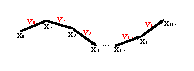
\includegraphics[width=2in]{../figures/trajectory.eps}
  \caption{An example streamline generated from a 2D distribution-based vector field is modeled as a sequence of vectors.}
  \label{trajectory}
\end{figure}

For the distribution-based vector fields, there is no unique streamline $v_{0:n}$ for a given starting point $x_0$. Let $\Omega_{x_0}$ be the set of all possible streamlines which originate from $x_0$ given the distribution-based data $\mathcal{H}$, we then can define a probability density function (pdf) over the path space, which is:
\begin{equation}
  p(v_{0:n}|\mathcal{H})
\end{equation}
where $\mathcal{H}$ is the set of observations from the distribution-based data along the streamline trajectory. Here, we denote the distribution obtained at the starting point $x_t$ of a vector $v_t$ as $\lambda_t=\mathcal{H}(v_t)$. By applying the Bayes theorem, the target distribution $p({v_{0:n}}|{\lambda_{0:n}})$ can be represented by the prior density $p({v_{0:n}})$ and the conditional observation density $p({\lambda_{0:n}}|{v_{0:n}})$, as:
\begin{equation}
  p({v_{0:n}}|{\lambda_{0:n}}) = \frac{{p({v_{0:n}})p({\lambda_{0:n}}|{v_{0:n}})}}{{p({\lambda_{0:n}})}}
\end{equation}
where ${p({\lambda_{0:n}})}$ is a normalizing constant for a fixed data realization, which equals to $\int {p({v_{0:n}},{\lambda_{0:n}})} d{v_{0:n}}$.

Scientific simulations commonly represent physical phenomena as continuous functions. Thus, streamlines integrated based on the data generated from such simulations are generically smooth. In the other words, the sequence of vector directions $v_{0:n}$ along the particle trace should transition smoothly when the step size $\Delta t$ is small enough. This constraint can be modeled as a conditional prior density $p({v_t}|{v_{0:t - 1}})$. In this paper, we assume the sequence $v_{0:n}$ forms a Markov chain, which means the vector direction $v_t$ only depends on the previous direction $v_{t-1}$, but not on $v_{t-2},...,v_0$; so:
\begin{equation}
  p({v_t}|{v_{0:t - 1}}) = p({v_t}|{v_{t - 1}})
\end{equation}
where $p({v_t}|{v_{t - 1}})$ denotes the probability density associated with the transition from $v_{t - 1}$ to $v_t$. Hence, the probability density for a given streamline can be formulated as:
\begin{equation}
  p({v_{0:n}}) = p({v_0})\prod\limits_{t = 1}^n {p({v_t}|{v_{t - 1}})}
\end{equation}
where $p(v_0)$ can be defined by a uniform distribution, since no prior knowledge is applied.

By measuring the observations $\lambda_{0:n}$ along a given streamline $v_{0:n}$, we can get the conditional observation density $p({\lambda_{0:n}}|v_{0:n})$, which defines a measure of how the observations match the given path. In the other word, the observation density gives how likely the distributions $\lambda_{0:n}$ will be observed if the given streamline $v_{0:n}$ actually exists in the flow field. Likewise, we assume that the observation measured at a point does not depend on any previous points in the trace, i.e.:
\begin{equation}
  p(\lambda_t|v_{0:t}) = p({\lambda_t}|{v_t})
\end{equation}
which defines the likelihood density:
\begin{equation}
  p({\lambda_{0:n}}|{v_{0:n}}) = \prod\limits_{t = 0}^n {p({\lambda_t}|{v_t})}
\end{equation}

By substituting (5) and (7) into (3), the posterior density $p({v_{0:n}}|{\lambda_{0:n}})$ can be expanded as:
\begin{equation}
  p({v_{0:n}}|{\lambda_{0:n}}) = \frac{{p({v_0})\prod\limits_{t = 1}^n {p({v_t}|{v_{t - 1}})} \prod\limits_{t = 0}^n {p({\lambda_t}|{v_t})} }}{{p({\lambda_{0:n}})}}
\end{equation}

\subsection{Local Modeling}

Based on equation (8), the key components of the posterior density $p({v_{0:n}}|{\lambda_{0:n}})$ are the prior density ${p({v_t}|{v_{t - 1}})}$ and the observation density ${p({\lambda_t}|{v_t})}$. In this section, we will elaborate how to model and estimate these two local densities in detail.

\subsubsection{Prior Density}

Prior density characterizes the relationship between two adjacent vector directions, which prefers to continue in the previous direction and gives decreasing probability for sharper turns. As presented by Zhang et al. in~\cite{Zhang20095}, the von Mises-Fisher distribution~\cite{fisher} has been selected as the prior density due to its mathematical simplicity and tractability. Some other common choices in the literature are the Watson distribution and the Kent distribution.

For a random $d$-dimensional unit vector $v$ on the $(d-1)$-dimensional sphere, with respect to the mean direction $\mu$ and the concentration parameter $\kappa$, the probability density function of the von Mises-Fisher distribution is given by
\begin{equation}
  f_{d}(v| \mu, \kappa)=C_{d}(\kappa)\exp \left( {\kappa \mu^T v } \right)
\end{equation}
where the normalization constant $C_{d}(\kappa)\,$ is
\begin{equation}
  C_{d}(\kappa)=\frac {\kappa^{d/2-1}} {(2\pi)^{d/2}I_{d/2-1}(\kappa)} \,
\end{equation}
in which $I_{d/2-1}$ denotes the modified Bessel function of the first kind and order $d/2-1$.

The parameter $\kappa$ defines in range $\kappa \ge 0$ is used to control the concentration of the distribution around the mean direction $\mu$. The distribution with higher concentration will have a greater $\kappa$ value. For example, the distribution is focused on a point of the sphere defined by $\mu$ for $\kappa  = \infty$, and is uniform on the sphere for $\kappa=0\,$. Figure~\ref{fisher} gives examples of points sampled from 2-dimensional von Mises-Fisher distributions with different $\kappa$.

\begin{figure}[htb!f]
  \centering
  \begin{subfigure}[b]{0.16\textwidth}
    \centering
    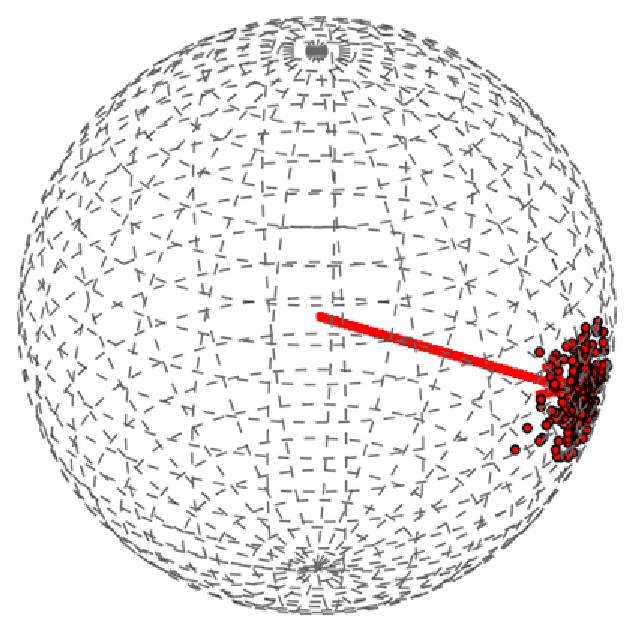
\includegraphics[width=0.9in]{../figures/vf_100.eps}
    \caption{$\kappa=100$}
  \end{subfigure}~
  \begin{subfigure}[b]{0.16\textwidth}
    \centering
    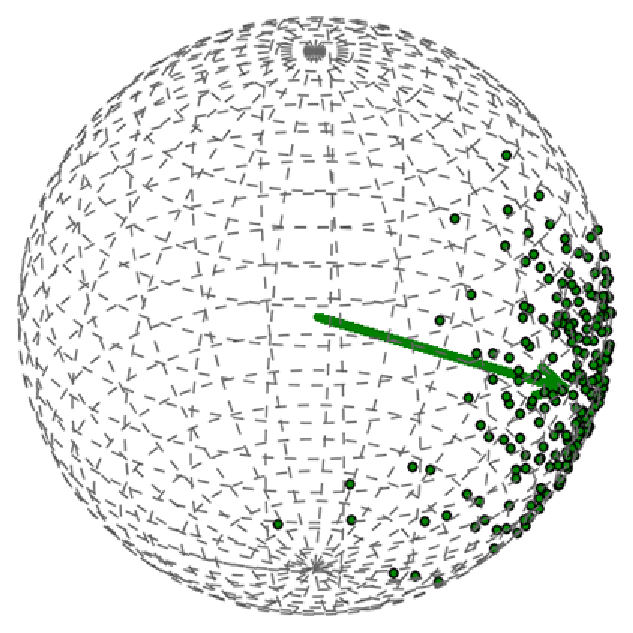
\includegraphics[width=0.9in]{../figures/vf_10.eps}
    \caption{$\kappa=10$}
  \end{subfigure}~
  \begin{subfigure}[b]{0.16\textwidth}
    \centering
    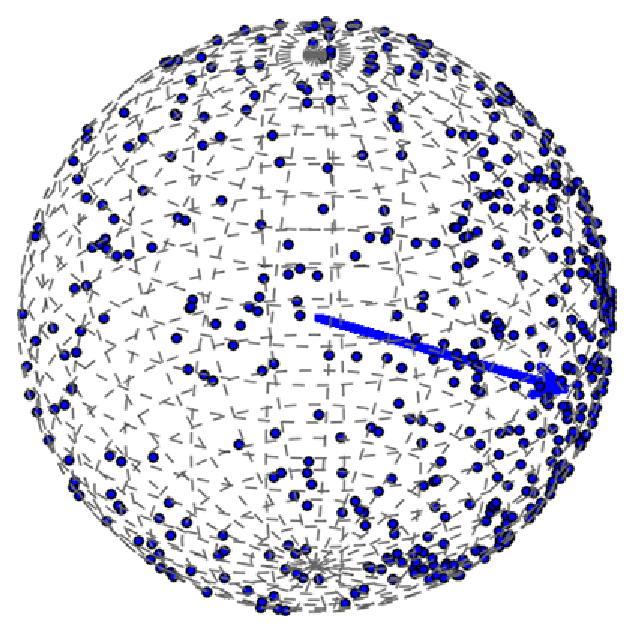
\includegraphics[width=0.9in]{../figures/vf_1.eps}
    \caption{$\kappa=1$}
  \end{subfigure}
  \caption{Points sampled from three von Mises-Fisher distributions on $2$-dimensional spheres with different value of $\kappa$. The mean directions are shown as arrows.}
  \label{fisher}
\end{figure}

In this work, the mean direction $\mu$ of the prior density is given by the previous vector direction ${v_{t - 1}}$. The concentration parameter $\kappa$ is given manually as a constant value. Thus, the prior density $p({v_t}|{v_{t - 1}})$ is defined by the von Mises-Fisher distribution with the mean direction ${v_{t - 1}}$ and the concentration parameter $\kappa$:
\begin{equation}
  p({v_t}|{v_{t - 1}}) = {f_d}({v_t}|{v_{t - 1}}, \kappa)
\end{equation}

\subsubsection{Observation Density}
